\documentclass[conference,a4paper]{APSIPA2026}
\usepackage{cite}
\usepackage{amsmath,amssymb,amsfonts}
\usepackage{graphicx}
\usepackage{textcomp}
\usepackage{xcolor}
\definecolor{figblue}{RGB}{37,84,160}
\definecolor{figred}{RGB}{198,58,45}
\usepackage{booktabs}
\usepackage{array}
\usepackage{multirow}
\usepackage{tikz}
\usetikzlibrary{shapes.geometric,arrows.meta,positioning,calc}
\usepackage{url}
\usepackage{geometry}
\geometry{a4paper, top=19mm, bottom=43mm, right=13mm, left=13mm}
\usepackage{fancyhdr}
\renewcommand{\headrulewidth}{0pt}
\renewcommand{\footrulewidth}{0pt}
\fancypagestyle{firststyle}{%
  \fancyhf{}%
  \fancyhead[C]{2026 Asia Pacific Signal and Information Processing Association Annual Summit and Conference (APSIPA ASC)}%
}
\usepackage[hidelinks]{hyperref}
\graphicspath{{figs/}}
% Float placement: keep every figure and table inside the section that declares
% it. The defaults reserve so much of each column for text that a dense paper
% defers floats across section boundaries.
\renewcommand{\topfraction}{0.92}
\renewcommand{\bottomfraction}{0.85}
\renewcommand{\textfraction}{0.06}
\renewcommand{\floatpagefraction}{0.72}
\setcounter{topnumber}{3}
\setcounter{bottomnumber}{2}
\setcounter{totalnumber}{5}
% Tighten the space reserved around floats: this paper is float-dense, and the
% class defaults reserve ~20pt above and below each one.
\setlength{\textfloatsep}{8pt plus 2pt minus 2pt}
\setlength{\floatsep}{8pt plus 2pt minus 2pt}
\setlength{\intextsep}{8pt plus 2pt minus 2pt}
\setlength{\dblfloatsep}{8pt plus 2pt minus 2pt}
\setlength{\dbltextfloatsep}{10pt plus 2pt minus 2pt}

\begin{document}

\title{An 8-bit Deep Learning Accelerator for GAN Image Generation on GF180MCU}

\author{
\IEEEauthorblockN{William Anthony, I~Made~Medika~Surya~W.M., John~Ruben~Saragi, Mahardhika~Putra~Adipratama,\\
Fairuz~Aquilla~Rahagi, Trio~Adiono, and Infall~Syafalni}
\IEEEauthorblockA{Bandung Institute of Technology, Bandung, Indonesia \\
E-mail: \{13223048, 13222021, 13222049, 13222081, 13222107\}@mahasiswa.itb.ac.id, \\
tadiono@itb.ac.id, infall@ieee.org}
}

\maketitle
\thispagestyle{firststyle}
\pagestyle{empty}

\begin{abstract}
This paper presents an 8-bit deep learning accelerator for a small MNIST GAN image generator, hardened through a fully open-source flow on the open GF180MCU 180~nm process. A quantized three-layer MLP generator maps onto a structural $4\times4$ processing-element array of native accumulation depth $K=256$. Where a folding predecessor stored the sixteen-accumulator result buffer in a small SRAM macro, this design realizes it as a register file --- cheaper and faster for a buffer the array geometry fixes at 48 bytes --- removing the last non-bandwidth macro and leaving \textbf{eight} $256\times8$ SRAM macros on a rectangular $1600\times1100~\mu$m die, with single-cycle reads and 16-cycle writeback. Antenna closed on a two-lever path: the roomy floorplan left four marginal violations on long SRAM-to-array broadcast nets, which clustering the eight macros shortened at the source, and a density sweep then routed to zero ($4\rightarrow2\rightarrow0$), reproducibly. The design is verified with a Universal Verification Methodology (UVM) environment in pyuvm on cocotb --- transaction-level, self-checking, with an independent reference model --- and signs off with zero DRC, LVS, XOR, and antenna violations at 40~ns across nine STA corners.
\end{abstract}

\begin{IEEEkeywords}
Deep learning accelerator, GF180MCU, SRAM macro, register file, antenna closure, UVM, cocotb, INT8 quantization, GAN, ASIC, LibreLane, open-source EDA.
\end{IEEEkeywords}

\section{Introduction}
Generative Adversarial Networks are a compact workload for testing neural inference on custom hardware. The generator used here is a small MNIST multi-layer perceptron turning a 64-dimensional latent vector into a $28\times28$ image; its arithmetic is dense matrix multiplication, so it maps onto a small array of multiply--accumulate units. An earlier version expressed this as behavioral loops and register memory arrays --- convenient for checking the algorithm, but not implementable, since buffers inferred as standard-cell registers make the design too large to route. It was restructured into a structural accelerator with a processing-element (PE) array, SRAM-backed buffers, and a controller, and hardened with eleven $256\times8$ SRAM macros on a $1600\times1500~\mu$m die.

This paper takes that design's memory question one step further. A folding predecessor had already reduced the result buffer to a single $64\times8$ macro storing 48 bytes in 64; but a buffer the array geometry fixes at sixteen 24-bit accumulators is small enough that even the shallowest SRAM macro is over-provisioned. Realized as a register file --- 384 flip-flops --- it removes that macro entirely, leaving only the eight operand macros the array bandwidth demands, and returns the buffer to single-cycle reads. The contributions are: (1)~a register-file result buffer that removes the last non-bandwidth macro and restores single-cycle access at negligible area; (2)~an antenna-closure path for a spread-out floorplan --- cluster the macros to shorten the broadcast nets at the source, then re-roll the marginal residue to zero with a density sweep --- confirmed reproducible by a byte-identical re-run; (3)~a Universal Verification Methodology environment, built open-source in pyuvm on cocotb, that checks the accelerator transaction-by-transaction against an independent reference model; and (4)~a full physical sign-off of the eight-macro rectangular die at 40~ns across nine STA corners.

\section{Related Work}
Most neural accelerators are arrays of multiply-and-accumulate units --- the systolic TPU \cite{tpu} at large scale, surveyed broadly in \cite{survey} --- and running a floating-point network on an integer array normally uses the per-tensor quantization scale of Jacob et al. \cite{jacob}. The fabricated reference points span three orders of magnitude: DianNao \cite{diannao}, Eyeriss \cite{eyeriss} with its row-stationary dataflow, and, closer to our scale, Wang et al. \cite{wang}, all closed-PDK designs on commercial nodes. The comparison that matters most is OpenSpike \cite{openspike}, a spiking accelerator in open SkyWater 130~nm with open EDA and OpenRAM memory: same open-flow premise, different workload and memory strategy (Table~\ref{tab:compare}). The workload is a pretrained MLP GAN \cite{goodfellow, ganpretrained}; the RTL builds on the open DLA Engine project \cite{dlaengine}.

\section{GAN Architecture}\label{sec:overview}

\begin{figure*}[!t]
\centering
\resizebox{\textwidth}{!}{%
\begin{tikzpicture}[x=1mm,y=1mm,
  outerblk/.style={draw=figblue,fill=figblue!4,rounded corners=2.5mm,line width=1pt},
  subblk/.style={draw=figblue!60,fill=white,rounded corners=1.6mm,line width=0.6pt},
  syn/.style={figblue!45,line width=0.3pt},
  flow/.style={-{Stealth[length=1.9mm,width=1.6mm]},figblue,line width=0.9pt},
  ax/.style={-{Stealth[length=1.2mm,width=1.1mm]},black!55,line width=0.4pt},
  fn/.style={figred,line width=1.1pt},
  ttl/.style={font=\scriptsize\bfseries,text=figblue!80!black},
  dim/.style={font=\tiny,text=black!60},
  cell/.style={draw=figblue!75!black,line width=0.35pt,minimum size=3.4mm,inner sep=0pt,font=\tiny}]
% ---- top-level blocks ----
\draw[outerblk] (0,-14) rectangle (19,14);
\draw[outerblk] (26,-15) rectangle (154,19);
\draw[outerblk] (161,-14) rectangle (181,14);
\node[font=\small\bfseries,text=figblue!80!black] at (90,16.1) {MLP GAN Generator};
% ---- fat arrows between top-level blocks ----
\draw[draw=figblue,fill=figblue!15,line width=0.8pt]
  (19.9,1.0) -- (23.2,1.0) -- (23.2,2.1) -- (25.3,0) -- (23.2,-2.1) -- (23.2,-1.0) -- (19.9,-1.0) -- cycle;
\draw[draw=figblue,fill=figblue!15,line width=0.8pt]
  (154.7,1.0) -- (158.0,1.0) -- (158.0,2.1) -- (160.1,0) -- (158.0,-2.1) -- (158.0,-1.0) -- (154.7,-1.0) -- cycle;
\node[dim] at (157.4,3.9) {reshape};
% ---- latent vector, drawn as a vector ----
\node[ttl,align=center] at (9.5,10.6) {Latent\\Vector};
\foreach [count=\i] \val/\sh in {0.8/45, -0.3/14, 1.2/60, -0.7/38}
  \node[cell,fill=figblue!\sh] at (9.5,{4.6-(\i-1)*3.4}) {$\val$};
\node[font=\tiny] at (9.5,-8.15) {$\vdots$};
\node[cell,fill=figblue!28] at (9.5,-10.6) {$0.5$};
\draw[line width=0.5pt,black!75] (7.2,6.6) -- (6.5,6.6) -- (6.5,-12.6) -- (7.2,-12.6);
\draw[line width=0.5pt,black!75] (11.8,6.6) -- (12.5,6.6) -- (12.5,-12.6) -- (11.8,-12.6);
\node[font=\scriptsize] at (9.5,-16.5) {$z\in\mathbb{R}^{64}$};
% ---- dense layers, drawn as neurons ----
\foreach \bx/\lin/\lout/\ltag in {29/64/256/L0, 71/256/256/L2, 113/256/784/L4}{
  \draw[subblk] (\bx,-13) rectangle (\bx+21,13);
  \node[ttl] at (\bx+10.5,10.2) {Dense \lout};
  \node[font=\tiny,text=black!45] at (\bx+2.6,10.9) {\ltag};
  \foreach \ly in {4.2,0,-4.2}
    \foreach \ry in {6.4,3.2,0,-3.2,-6.4}
      \draw[syn] (\bx+5.5,\ly) -- (\bx+15.5,\ry);
  \foreach \ly in {4.2,0,-4.2}
    \node[circle,draw=figblue!80!black,fill=figblue!22,inner sep=0pt,minimum size=3.2mm,line width=0.4pt] at (\bx+5.5,\ly) {};
  \foreach \ry in {6.4,3.2,0,-3.2,-6.4}
    \node[circle,draw=figblue!80!black,fill=figblue!22,inner sep=0pt,minimum size=2.8mm,line width=0.4pt] at (\bx+15.5,\ry) {};
  \node[font=\tiny] at (\bx+5.5,-7.2) {$\vdots$};
  \node[font=\tiny] at (\bx+15.5,-9.3) {$\vdots$};
  \node[dim] at (\bx+5.5,-11.3) {\lin};
  \node[dim] at (\bx+15.5,-11.3) {\lout};
}
% ---- activations, drawn as their functions ----
\foreach \cx/\aname in {60.5/ReLU, 102.5/ReLU, 144.5/Tanh}{
  \draw[subblk] (\cx-6.5,-13) rectangle (\cx+6.5,13);
  \node[ttl] at (\cx,10.2) {\aname};
  \draw[ax] (\cx-4.9,-1.4) -- (\cx+4.9,-1.4);
  \draw[ax] (\cx,-6.3) -- (\cx,3.5);
}
\foreach \cx in {60.5,102.5}{
  \draw[fn] (\cx-4.3,-1.4) -- (\cx,-1.4) -- (\cx+3.4,2.0);
  \node[dim] at (\cx,-8.7) {$\max(0,x)$};
}
\draw[fn,smooth,samples=29,domain=-4.3:4.3] plot ({144.5+\x},{-1.4+3.4*(exp(\x/0.75)-1)/(exp(\x/0.75)+1)});
\node[dim] at (144.5,-8.7) {$\tanh(x)$};
% ---- flow arrows between sub-blocks ----
\foreach \xa in {50.4,67.4,92.4,109.4,134.4}
  \draw[flow] (\xa,0) -- (\xa+3.2,0);
% ---- generated image ----
\node[ttl,align=center] at (171,10.6) {Generated\\Image};
\node[inner sep=0pt] at (171,-2.6) {
\includegraphics[width=12mm,height=12mm]{digit_seed6.jpg}};
\draw[black!60,line width=0.4pt] (165,-8.6) rectangle (177,3.4);
\node[font=\scriptsize] at (171,-16.5) {$28\times28$ grayscale};
\end{tikzpicture}}
\caption{MLP GAN generator: the 64-dimensional latent vector $z$ is expanded through two 256-neuron ReLU hidden layers and a 784-neuron tanh output layer into a $28\times28$ grayscale image.}
\label{fig:gan}
\end{figure*}


The generator (Fig.~\ref{fig:gan}) projects a 64-dimensional latent vector through two 256-neuron ReLU hidden layers into a 784-neuron tanh output layer, reshaped as a $28\times28$ grayscale image. Its dense layers are L0 ($256\times64$, ReLU), L2 ($256\times256$, ReLU), and L4 ($784\times256$, tanh): 282{,}624 MACs. At four output neurons per tile, L0 and L2 need 64 tiles each and L4 needs 196 --- 324 tiles per image.

\section{Hardware Architecture}\label{sec:hw}

The DLA computes a tiled matrix multiplication $C=A\times B$ with array size $N=4$ and native accumulation depth $K=256$, so one transaction accumulates a full 256-term dot product --- the inner dimension of the widest generator layers. $K$ is temporal: it sets how many cycles the same 16 PEs accumulate, not the array size. An earlier RTL revision defaulted to $K=4$ and relied on a harness override; since the physical flow synthesizes bare RTL defaults, the hardened default was widened to $K=256$, a parameter-only change as the operand SRAMs were already 256 deep. Per transaction the controller clears the accumulators, enables the array for $K$ cycles, and stores the result block to C through a writeback path that serializes the sixteen accumulators.

At the top level (Fig.~\ref{fig:top}) A provides one row vector to the array and B one column vector, the control unit generates the read index and the clear, enable, done, and busy signals, and the output bus carries the accumulated C values.

\begin{figure}[!ht]
\centering
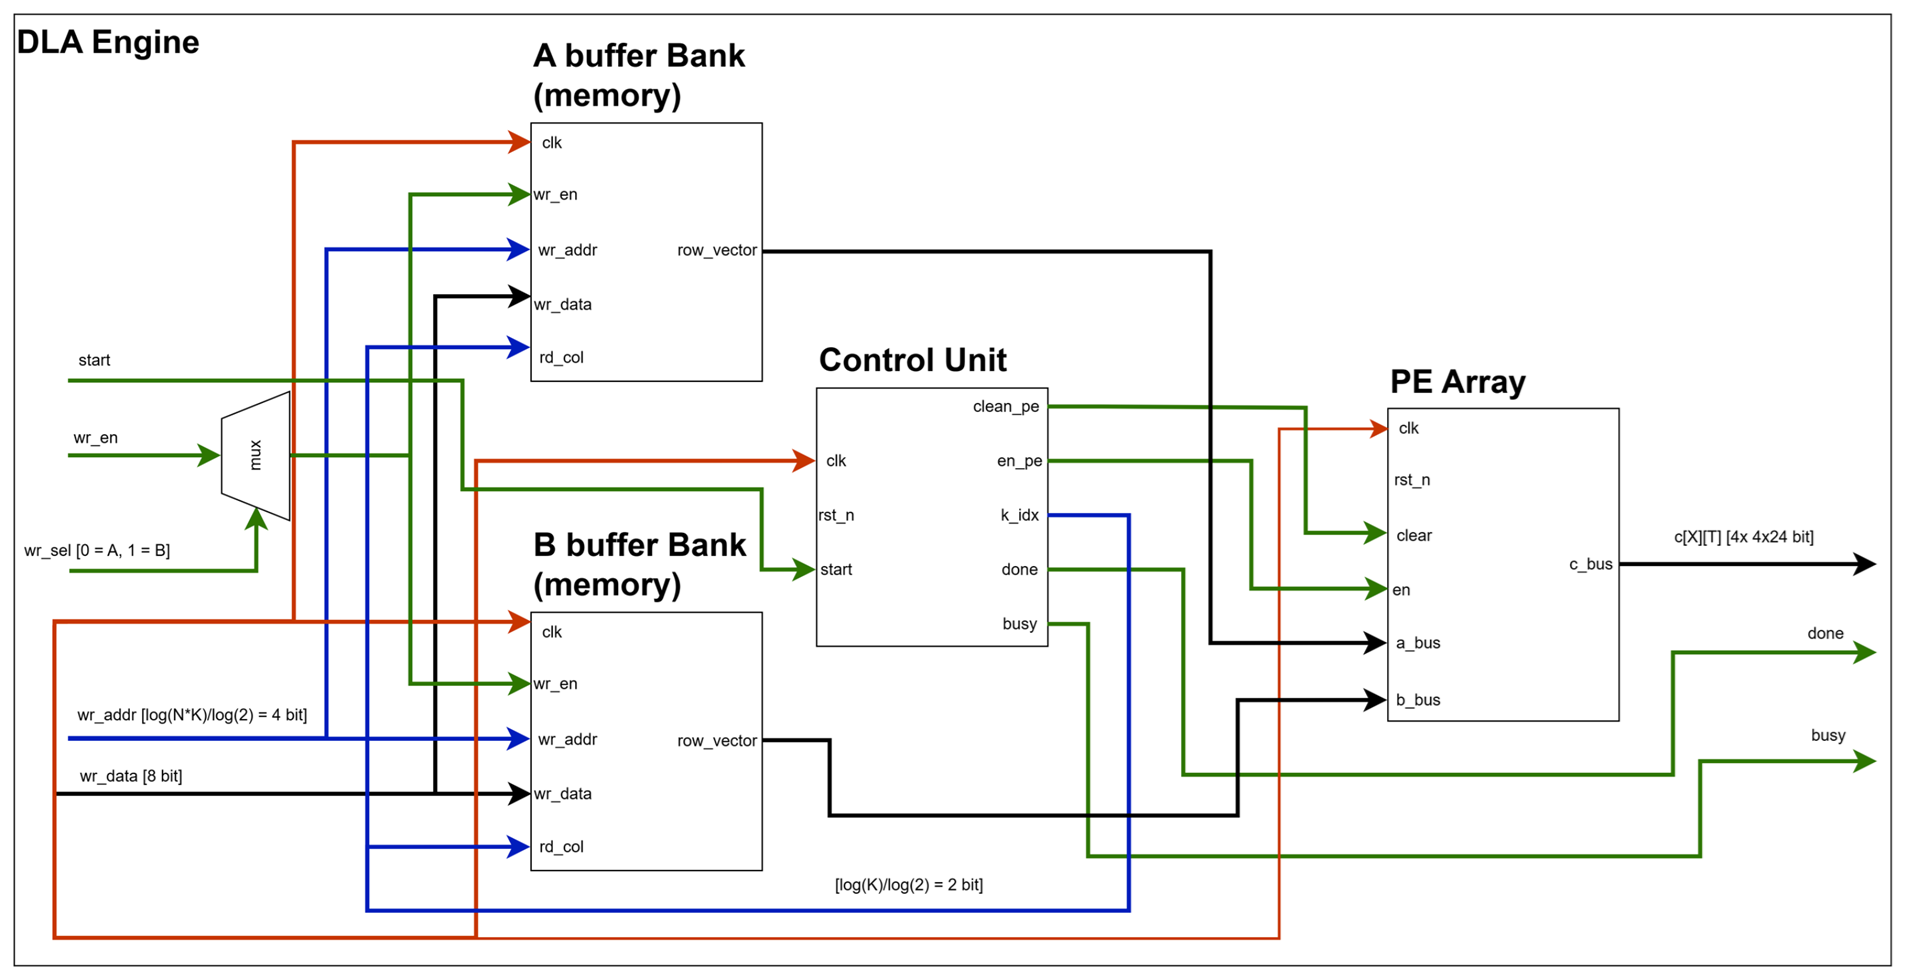
\includegraphics[width=0.98\columnwidth]{Top_level.png}
\caption{DLA engine top level.}
\label{fig:top}
\end{figure}

\subsection{PE Array and Controller}
Each PE (Fig.~\ref{fig:pe}, left) takes two signed 8-bit operands, multiplies them, sign-extends the 16-bit product to 24 bits, and adds it to a local accumulator,
\begin{equation}
acc[n]=acc[n-1]+a[n]\,b[n],
\end{equation}
so after $K$ cycles it holds one tile output; 24 bits give 256 accumulated 8-bit products enough range. The array (Fig.~\ref{fig:pe}, right) is 16 PEs in a $4\times4$ grid, each row fed one activation lane and each column one weight lane by broadcast, each PE accumulating locally --- output-stationary, all 16 in parallel, one tile per accumulation loop. The controller (Fig.~\ref{fig:fsm}) has four states: IDLE waits for START, CLEAR zeroes the accumulators, COMPUTE enables the array and increments the A and B addresses until all $K$ terms are consumed, DONE holds the completion flag until START falls. A writeback sequencer then serializes the accumulators into C and raises a writeback-done flag.

\begin{figure}[!ht]
\centering
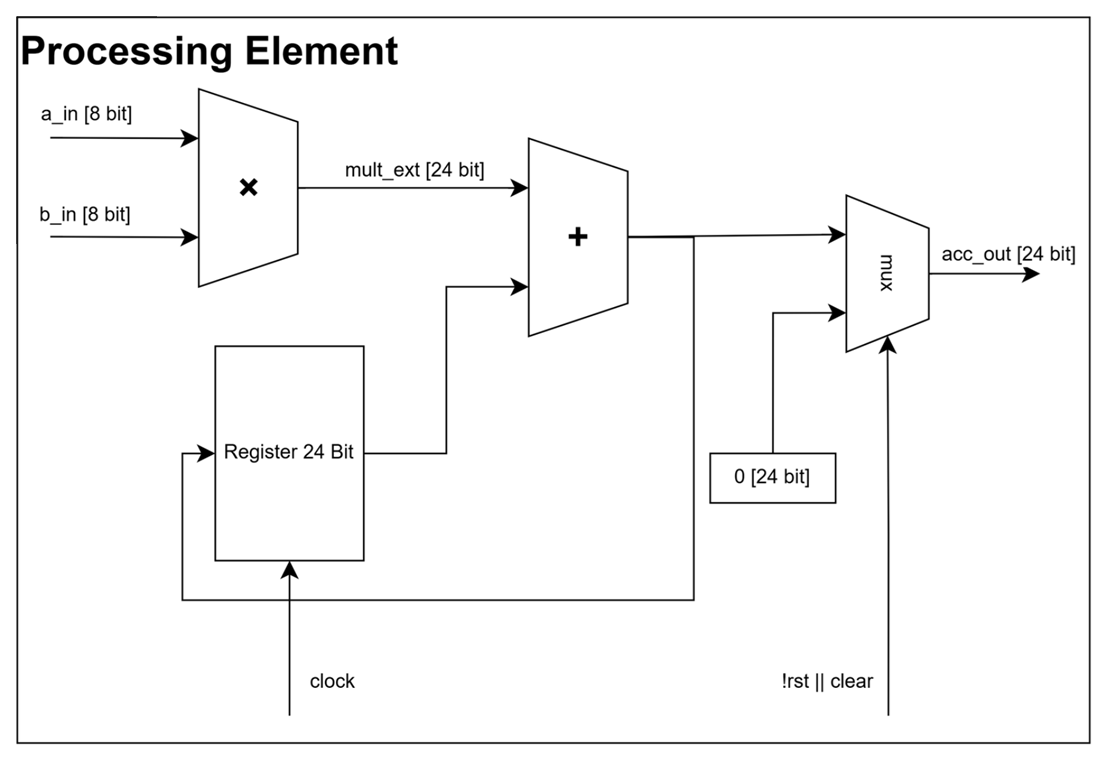
\includegraphics[width=0.46\columnwidth]{PE.png}\hfill
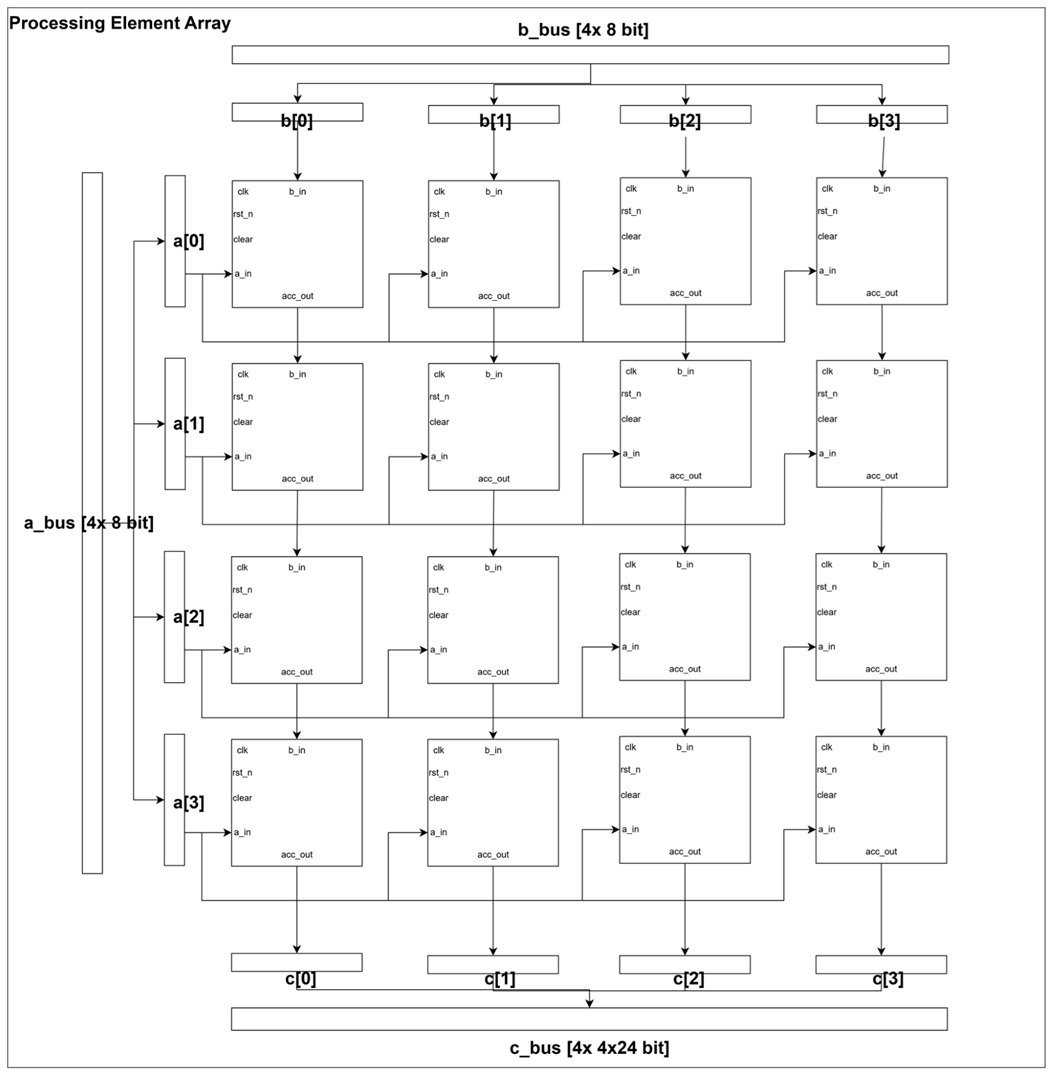
\includegraphics[width=0.50\columnwidth]{PE_Array.png}
\caption{Processing element datapath (left) and the $4\times4$ array (right).}
\label{fig:pe}
\end{figure}

\begin{figure}[!ht]
\centering
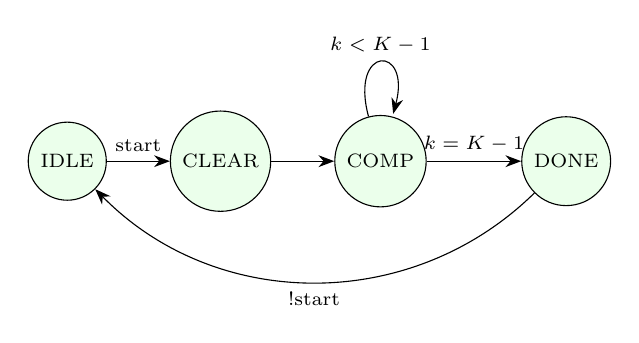
\begin{tikzpicture}[
  font=\scriptsize,>={Stealth[length=2mm]},
  st/.style={draw,circle,minimum size=9mm,fill=green!8}
]
\node[st] (idle) {IDLE};
\node[st,right=8mm of idle] (clear) {CLEAR};
\node[st,right=8mm of clear] (comp) {COMP};
\node[st,right=12mm of comp] (done) {DONE};
\draw[->] (idle) -- node[above]{start} (clear);
\draw[->] (clear) -- (comp);
\path (comp) edge[->,loop above] node{$k<K-1$} (comp);
\draw[->] (comp) -- node[above]{$k=K-1$} (done);
\draw[->] (done) to[bend left=45] node[below]{!start} (idle);
\end{tikzpicture}
\caption{Controller state machine.}
\label{fig:fsm}
\end{figure}

\subsection{Operand SRAMs and a Register-File Result Buffer}
The operand buffers are single-port SRAM macros: four $256\times8$ for A, one per row lane, and four for B, one per column. Eight is a bandwidth floor, not a capacity choice --- the array consumes four A and four B bytes per compute cycle from 1RW 8-bit parts, so no depth reduction reduces the count --- and both banks are exactly full at 1{,}024~bytes. In this design these eight are the \emph{only} macros on the die.

The result buffer is where the predecessors spent a macro and this design spends none. It holds $N\times N=16$ accumulators of 24 bits --- 48 bytes, a size the array geometry fixes forever. An eleven-macro ancestor stored it as three $256\times8$ byte-plane macros (203{,}314~$\mu$m$^2$); a nine-macro successor folded those onto one $64\times8$ macro (45{,}861~$\mu$m$^2$), at the cost of a four-cycle read and a 48-cycle writeback. Both still paid a macro's overhead --- keep-out halo, Metal3 power hookup, a fixed floorplan slot --- to hold 384 bits. This design holds the 384 bits in a register file: sixteen 24-bit words of flip-flops with a registered read, addressed as $\mathit{addr}=i\times N+j$, which synthesis places freely in the fabric, so the ninth macro disappears. It is smaller and faster than the folded macro it replaces --- roughly 400 flip-flops and a $16{:}1$ multiplexer, on the order of $10^4~\mu$m$^2$ against 45{,}861 --- with a one-cycle write (writeback returns to 16 cycles from 48) and a next-cycle read. A buffer this small, fixed in size and off the critical path, is exactly where a register file dominates a hard macro on area, latency, and floorplan simplicity at once. The operand-SRAM wrapper is unchanged, and the one-cycle operand read is still absorbed by delaying the PE enable one cycle.

\section{Chip-Level Integration}\label{sec:chip}

The accelerator exposes 53 signal bits, but the shuttle slot gives only 20 general-purpose digital pads beside 60 analog, 8 supply, clock, and reset pads. Rather than a pin-per-signal map, the core wraps the accelerator behind a synchronous 4-wire serial bridge (SCLK, MOSI, CS\_N, MISO) that treats SCLK as data: all three inputs are double-flop synchronized and SCLK edge-detected, avoiding a second clock domain. Frames shift MSB-first while CS\_N is low --- 2-bit command, 10-bit address, plus 8 data bits on writes: WRITE\_A and WRITE\_B load the operand buffers, START launches a tile, READ\_C returns a 24-bit two's-complement result on MISO, and a rising CS\_N aborts safely. Three status flags (busy, done, writeback-done) drive pads directly for scope-visible liveness, so 9 of the slot's 91 pads are used. The register-file result buffer also simplifies the host protocol: READ\_C returns on the cycle after its address, so the host needs none of the plane-walk delay the folded-macro ancestor imposed, whose three-plane read forced extra idle core clocks before the data.

The padring is the wafer.space GF180MCU template \cite{padring} for a $2935\times2935~\mu$m workshop slot. It shorts the pad and core supplies into one rail on every pad, so the chip is single-supply by construction, and the operating point is 3.3~V for the whole die: logic and SRAM are 3.3~V parts and the foundry I/O cells are characterized at 3.3~V, so every cell runs in a foundry-characterized corner and the I/O levels suit a 3.3~V microcontroller host directly. A predecessor completed this flow with a clean chip-level sign-off, LVS over 71{,}668 instances included; the padring slot is a fixed, shared frame, so \textbf{it has not been re-run against the eight-macro macro}, which is the reason this paper reports macro-level results.

\section{Software to Hardware Flow}\label{sec:sw}

The hardened core is the DLA engine alone; everything around it is a host (Fig.~\ref{fig:hwsoft}). In simulation that is Python plus a Verilog testbench preparing quantized weights, inputs, and reference outputs; on the finished chip, a microcontroller streaming the same tile schedule over the serial protocol.

\begin{figure}[!ht]
\centering
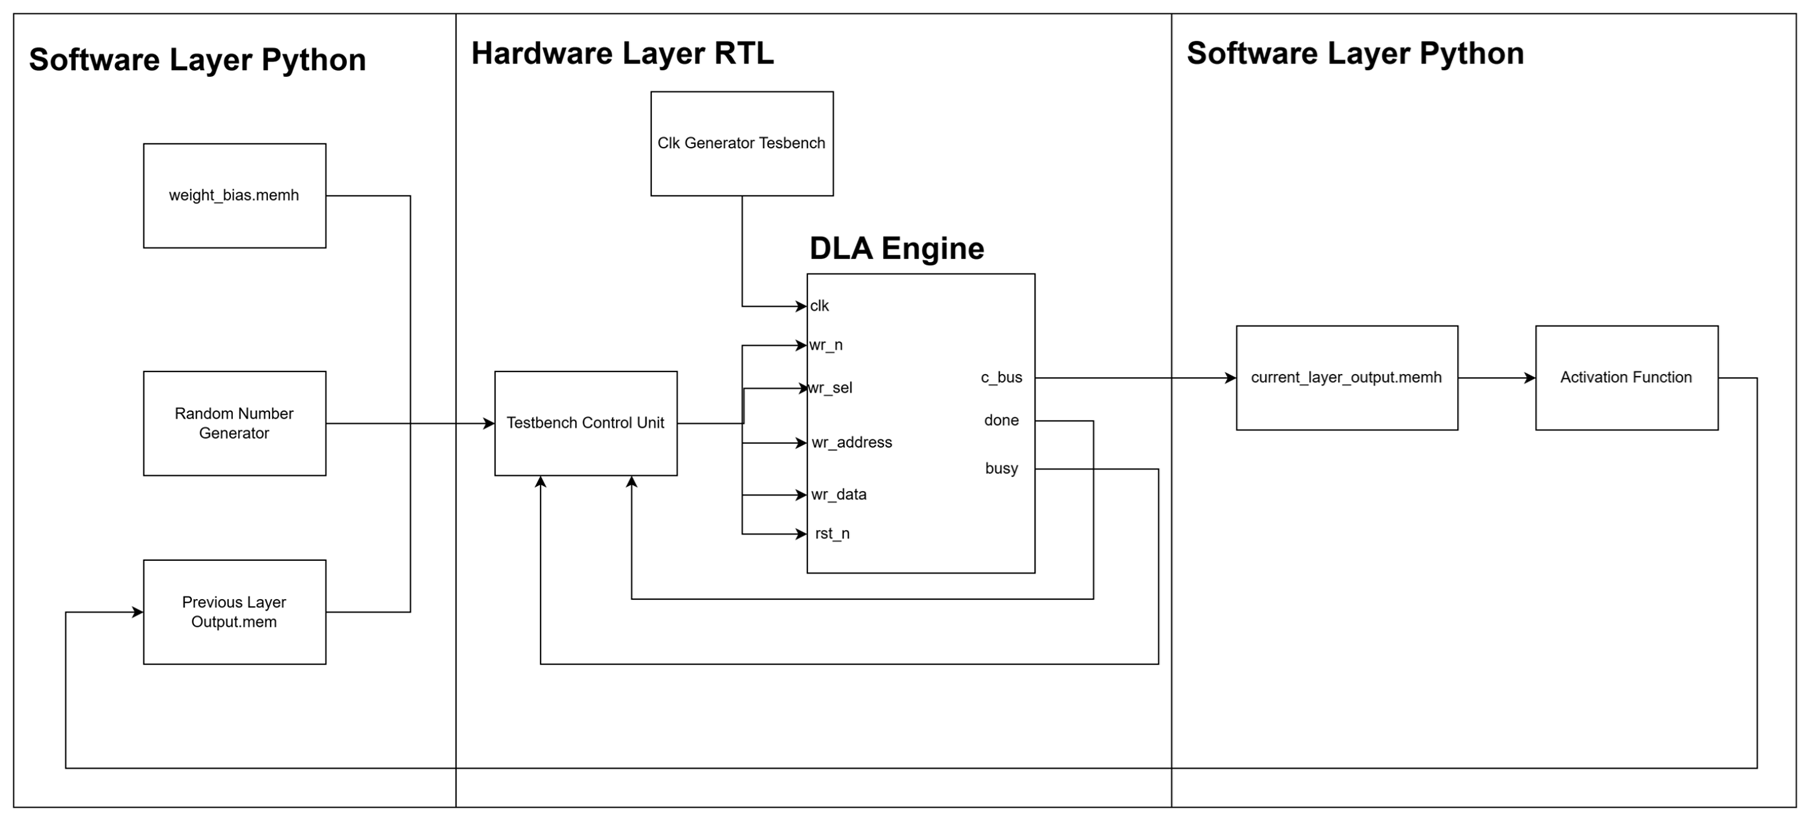
\includegraphics[width=0.94\columnwidth]{Hardware_Software_Integration.png}
\caption{Hardware and software flow.}
\label{fig:hwsoft}
\end{figure}

\subsection{Quantization and Requantization}
Every weight and bias tensor becomes signed 8-bit with one scale factor per tensor, taken from its largest absolute value and recorded in a manifest the testbench reuses. The DLA returns only a tile's integer dot product; the surrounding math is integer on the host, so hardware matches the Python reference exactly. Hidden-layer results are rescaled, biased, ReLU-activated, and requantized to 8 bits; output-layer results go to fixed point, through a tanh lookup table, to a grayscale pixel.

\subsection{Why INT8}\label{sec:format}

\begin{table}[!ht]
\caption{Numeric formats: accuracy against an exact FP64 render (10 latents, 7{,}840 pixels), and hardware cost. PE area is synthesized on the 3.3~V cells; accumulator width is what 256 accumulated products need.}
\label{tab:format}
\centering
\renewcommand{\arraystretch}{1.0}
\begin{tabular}{@{}lcccrc@{}}
\toprule
 & \multicolumn{2}{c}{Pixel error (gray levels)} & Weights & PE area & Acc. \\
\cmidrule(lr){2-3}
Format & mean & max & (KiB) & ($\mu$m$^2$) & (bits) \\
\midrule
INT4   & 22.26 & 255 & 138 & 6{,}245  & 15 \\
\textbf{INT8}  & \textbf{1.22} & \textbf{72} & \textbf{276} & \textbf{15{,}963} & \textbf{23} \\
INT16  & 0.01  & 1   & 552 & 47{,}037 & 39 \\
FP16   & 0.06  & 5   & 552 & ---      & --- \\
\bottomrule
\end{tabular}
\end{table}
Operand width sets multiplier area, buffer depth, and stream volume at once, so it was chosen by measurement: each format was applied to the same FP32 checkpoint and its render compared against an exact FP64 render of the same latent, against one PE's synthesized area at that width (Table~\ref{tab:format}). INT4 is not viable --- a per-tensor scale leaves seven magnitude steps, and 256 accumulated terms of that coarseness destroy the digit. INT16 is essentially exact but costs $2.95\times$ the PE area, a 39-bit accumulator, and double the weight traffic, which doubles time per image since streaming dominates latency (Section~\ref{sec:perf}). FP16 is no more accurate than INT16 for the same memory and a different datapath; none was built, so no area is quoted. INT8 sits at the knee: 1.2 gray levels of mean error is invisible in a $28\times28$ digit, the 16-bit product fits the 24-bit accumulator, and the width matches the SRAM word, so buffers need no packing logic.

\section{Verification}\label{sec:map}

The generator maps onto the DLA as tiled dense layers: per tile the four weight rows go to A and the shared input vector to B, the array performs the dot products, and the results land in C, one datapath serving every layer.

\subsection{Golden-Vector Regression}
A directed suite passes against Python golden vectors: a GEMM on a single lane; a full $N{=}4$/$K{=}256$ tile exercising every A and B macro; one layer row; a full 784-pixel image; and the pad-level serial protocol driven as external hardware would. Because the result buffer is now a register file, the read-timing complications the folded macro imposed on every caller --- a plane-walk restart on address change, an extra wait cycle in the serial bridge --- disappear: a read is simply valid on the next cycle, the same contract as the operand SRAMs.

\subsection{UVM Verification}
Beyond directed vectors, the accelerator is verified with a Universal Verification Methodology (UVM, IEEE~1800.2) environment. UVM is normally SystemVerilog on a commercial simulator; to keep the flow open-source, the environment is built in \emph{pyuvm}, a faithful re-implementation of the UVM class library, driving the design through cocotb over Icarus Verilog, so every component has its SystemVerilog counterpart. The hierarchy is standard (Fig.~\ref{fig:uvm}): a \emph{sequence} generates transactions, each a full $A\times B$ tile with random signed operands; a \emph{sequencer} and \emph{driver} apply them at the pins --- load A and B, pulse START, read the sixteen results; a passive \emph{monitor} reconstructs the observed result matrix from the read-back bus; and a \emph{scoreboard} predicts $C=A\times B$ with an independent 24-bit integer reference model and compares. Everything above the driver speaks in transactions rather than pin values, decoupling stimulus and checking from the protocol. A directed all-ones tile ($C_{ij}=K=256$) and constrained-random tiles all pass, sixteen outputs each. The value of the UVM layer over directed vectors is structural: the scoreboard's reference is independent of the stimulus, the monitor observes the true output pins as a black box, and adding coverage or new sequences needs no change to the checker --- the reusability directed testbenches lack.

\begin{figure}[!ht]
\centering
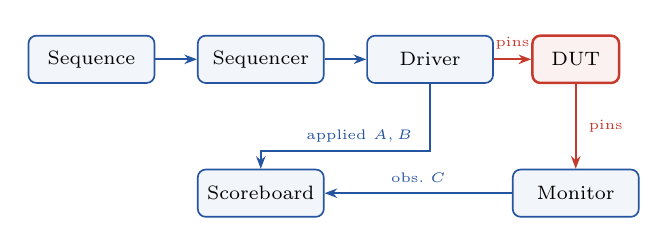
\begin{tikzpicture}[x=1cm,y=1cm,font=\scriptsize,>={Stealth[length=1.7mm]},
  blk/.style={draw=figblue,fill=figblue!6,rounded corners=1mm,line width=0.6pt,
    minimum height=6mm,minimum width=16mm,align=center,inner sep=1pt},
  dut/.style={draw=figred,fill=figred!7,rounded corners=1mm,line width=0.9pt,
    minimum height=6mm,minimum width=11mm,align=center},
  tx/.style={-{Stealth[length=1.6mm]},figblue,line width=0.7pt},
  pin/.style={-{Stealth[length=1.6mm]},figred,line width=0.8pt}]
\node[blk] (seq) at (0,1.7)    {Sequence};
\node[blk] (sqr) at (2.15,1.7) {Sequencer};
\node[blk] (drv) at (4.3,1.7)  {Driver};
\node[dut] (dut) at (6.15,1.7) {DUT};
\node[blk] (mon) at (6.15,0)   {Monitor};
\node[blk] (sb)  at (2.15,0)   {Scoreboard};
\draw[tx]  (seq) -- (sqr);
\draw[tx]  (sqr) -- (drv);
\draw[pin] (drv) -- (dut) node[midway,above,font=\tiny]{pins};
\draw[pin] (dut) -- (mon) node[midway,right=1pt,font=\tiny]{pins};
\draw[tx]  (mon) -- (sb)  node[midway,above,font=\tiny]{obs.\ $C$};
\draw[tx]  (drv.south) -- ++(0,-0.85) -| (sb.north);
\node[font=\tiny,text=figblue] at (3.4,0.72) {applied $A,B$};
\end{tikzpicture}
\caption{UVM environment: stimulus flows as transactions from the sequence to the driver, which applies it at the pins; the monitor reconstructs the result and the scoreboard checks it against an independent reference model fed the applied operands.}
\label{fig:uvm}
\end{figure}

\subsection{Gate-Level and End-to-End}
Gate-level re-simulation on the routed eight-macro netlist --- inserted buffers and roughly 10{,}000 antenna diodes included --- reproduces the golden results bit-exactly, closing the gap between correct RTL and a correct taped-out netlist. The rendered digits (Fig.~\ref{fig:samples}) are limited by the small generator and INT8 quantization but confirm the full software-to-hardware path runs end to end.

\begin{figure}[!ht]
\centering

\includegraphics[width=0.15\linewidth]{digit_seed6.jpg}\hspace{3mm}

\includegraphics[width=0.15\linewidth]{digit_seed5.jpg}\hspace{3mm}
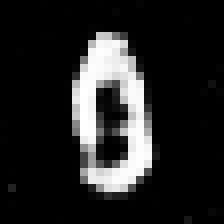
\includegraphics[width=0.15\linewidth]{digit_seed9.jpg}
\caption{Digits generated through the hardware path.}
\label{fig:samples}
\end{figure}

\section{Physical Implementation}\label{sec:phys}

The design is implemented with LibreLane \cite{librelane} on the GF180MCU open PDK \cite{gf180pdk}, hardened as a macro whose GDS/LEF/liberty views a padring integration consumes; everything below is that macro.

\subsection{Single-Supply 3.3~V Library Migration}
The buffer SRAM \cite{gf180sram} is a 3.3~V IP but the open PDK ships only 5~V cells, so a first version mixed a 5~V core with 3.3~V SRAMs --- fine for layout checks, level-shifted on silicon. Migrating to the third-party \texttt{gf180mcu\_as\_sc\_mcu7t3v3} native-3.3~V library, which ships nine liberty corners and a LibreLane integration, makes the die single-supply; bring-up surfaced three bugs in its flow integration (a missing timing-corner variable, a synthesis-exclusion filename mismatch, and non-synthesizable \texttt{\$random} initializers in six sequential-cell models that crashed lint), all fixed at the library source. The 3.3~V cells are far faster than the 5~V ones: the first run at 75~ns closed with $+44$~ns of setup slack, so the clock was retimed to 40~ns (25~MHz).

\subsection{Hardening the Accelerator Macro}

\begin{table}[!ht]
\caption{Antenna closure on the eight-macro die (40 ns, $1600\times1100~\mu$m). All runs are DRC-, LVS-, and timing-clean; only antenna varies. Violating nets are long SRAM-to-array broadcast and buffer-fanout nets.}
\label{tab:antenna}
\centering
\renewcommand{\arraystretch}{1.0}
\begin{tabular}{@{}llccl@{}}
\toprule
Placement & Density & Nets & Worst & Note \\
\midrule
roomy grid          & 56 & 4 & $1.44\times$ & baseline \\
roomy, margin 40    & 56 & 4 & $1.44\times$ & diodes no help \\
\midrule
cluster $55~\mu$m   & 48 & 2 & $1.26\times$ & broadcast shortened \\
cluster $55~\mu$m   & 44 & 1 & ---          & sweep \\
\textbf{cluster $55~\mu$m} & \textbf{50} & \textbf{0} & --- & \textbf{sign-off} \\
cluster $55~\mu$m   & 52 & 2 & ---          & sweep \\
\bottomrule
\end{tabular}
\end{table}
Four configuration points were essential: a synthesis define keeps the SRAM a hard macro (without it the memory is silently built from flip-flops); the eight macros are placed explicitly; the SRAM power pins reach only Metal3, so the macro power connection is made there; and routing runs to Metal5, with cell padding for diode access and diodes inserted at placement, in-router repair disabled --- its verification reroute aborts on clock-net diode pin access.

Antenna closure on the eight-macro floorplan took a different path from the folding predecessor's (Table~\ref{tab:antenna}). Laid out first on a roomy $1600\times1100~\mu$m die with the macros spread evenly, the design signed off clean except for four marginal antenna violations (worst $1.44\times$), all on long SRAM-to-array broadcast nets: with the macros far apart, a row or column broadcast crossed a large fraction of the die. Two levers were tried in isolation. Raising the pre-route diode margin left the count at four --- extra diodes cannot shorten a wire, so a length-dominated violation is unmoved. Clustering the eight macros into a compact central $4\times2$ block (channels tightened to $55~\mu$m) attacked the cause instead: the placer packs the datapath logic against the clustered memories, so the broadcast nets shrink, and the count fell to two. A density sweep over the clustered floorplan then re-rolled the last two marginal fanout nets: densities of 44, 48, 50 and 52 gave one, two, \textbf{zero}, and two violations, non-monotonically, and 50 reached zero. The result reproduces --- an independent re-run produced a byte-identical placement-and-routing database --- so it is a found configuration, not a routing-thread fluke.

The lesson generalizes: antenna on this flow is a placement problem, not a repair-tool one --- shorten the offending nets, whether by moving one mis-placed macro (as the nine-macro predecessor did) or by clustering all of them, then let a density perturbation route the marginal residue clean.

\begin{figure}[!ht]
\centering
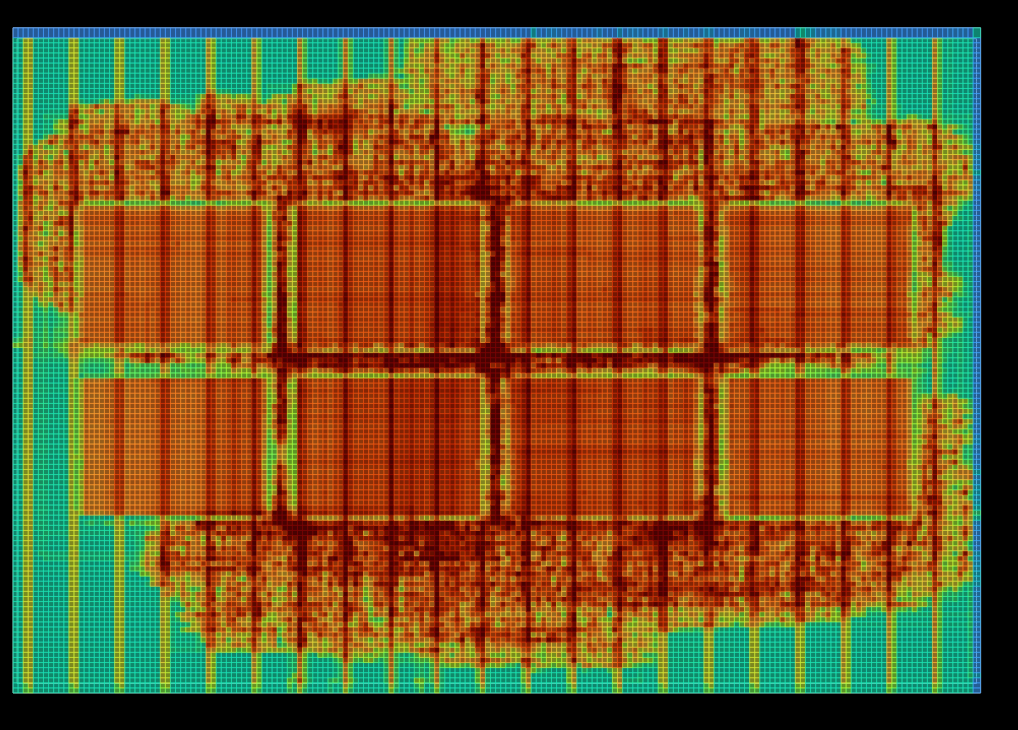
\includegraphics[width=0.485\columnwidth]{Longtin_Heat.png}\hfill
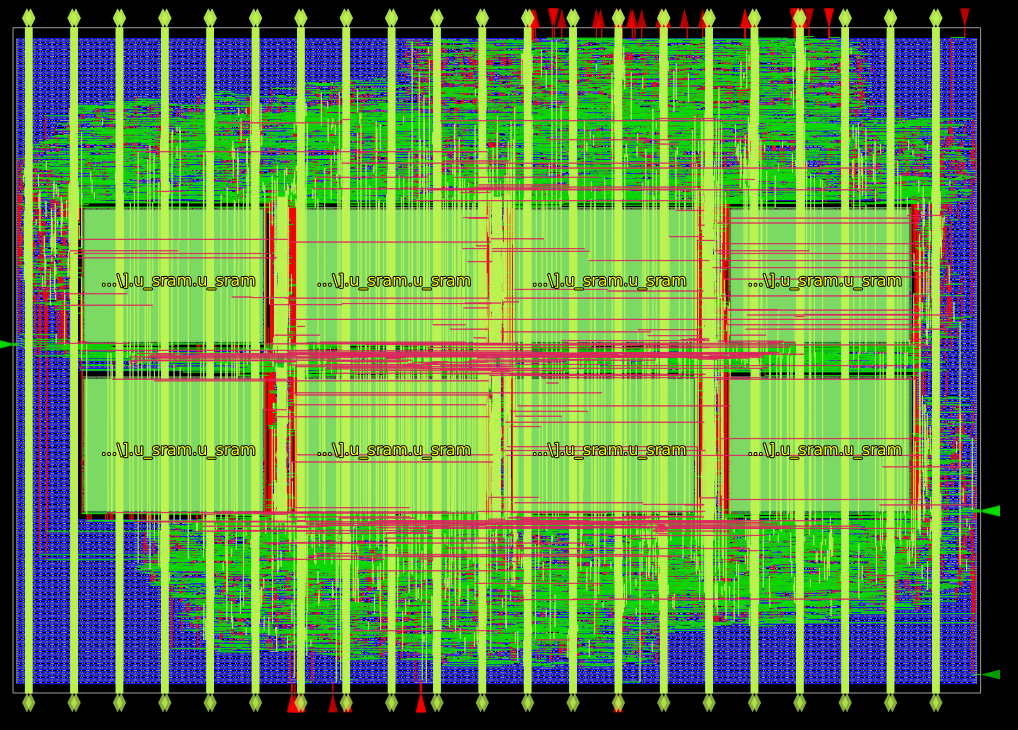
\includegraphics[width=0.485\columnwidth]{Longtin_OR.png}
\caption{Hardened macro, $1600\times1100~\mu$m: placement-density heatmap (left; red packed, blue empty) and the place-and-route view (right, macros labeled). The eight SRAM macros cluster into a central $4\times2$ block --- four A on the lower row, four B on the upper --- and the datapath logic packs against them, keeping the SRAM-to-array broadcast nets short; the result buffer is a register file, not a macro.}
\label{fig:layout}
\end{figure}

Fig.~\ref{fig:layout} shows the resulting layout and Table~\ref{tab:vs9} the sign-off: zero Magic DRC errors, zero Netgen LVS errors over 23{,}540 devices, zero GDS XOR differences, zero violating antenna nets and pins, and the 40~ns clock met at all nine STA corners. Static IR-drop analysis reports a worst on-die supply droop of $0.80$~mV on VSS and $0.35$~mV on VDD against 3.3~V with zero power-grid violations --- read as the on-die grid only, since a core macro carries no package or pad model. The nominal 121~mW is almost entirely internal power estimated with the flow's default switching activity, and should be read as a conservative tool estimate rather than a measurement.

\subsection{Area and Timing Detail}\label{sec:areatiming}

\begin{table}[!ht]
\caption{Sign-off of the eight-macro register-buffered design against the nine-macro folded-buffer predecessor. Both are hardened on GF180MCU 180~nm at 3.3~V with the \texttt{gf180mcu\_as\_sc\_mcu7t3v3} cells at 40~ns, and both close with 0 DRC, 0 LVS, 0 XOR, and 0 antenna violations. Power is a tool estimate.}
\label{tab:vs9}
\centering
\renewcommand{\arraystretch}{1.0}
\begin{tabular}{@{}lrrr@{}}
\toprule
 & 9 macros & 8 macros & Change \\
\midrule
Die ($\mu$m)            & $1375{\times}1325$ & $1600{\times}1100$ & \\
Die area (mm$^2$)       & 1.822   & 1.760   & $-3\%$ \\
Core area (mm$^2$)      & 1.761   & 1.692   & $-4\%$ \\
SRAM macros             & 9       & 8       & $-1$ \\
C buffer                & $64{\times}8$ macro & register file & \\
C buffer area ($\mu$m$^2$) & 45{,}861 & $\sim$10{,}000 & std cells \\
Instances               & 79{,}676 & 84{,}875 & $+7\%$ \\
Power (mW)              & 133     & 121     & $-9\%$ \\
Wirelength (mm)         & 812     & 997     & $+23\%$ \\
Writeback (cycles)      & 48      & 16      & $-67\%$ \\
C read latency (cycles) & 4       & 1       & $-75\%$ \\
Compute per image (ms)  & 3.95    & 3.54    & $-10\%$ \\
Setup slack, worst (ns) & $+16.24$ & $+15.74$ & \\
Hold slack, worst (ns)  & $+0.116$ & $+0.118$ & \\
\bottomrule
\end{tabular}
\end{table}

The core stays memory-dominated: eight macros take $0.542$~mm$^2$ (32\% of the core), a bandwidth floor with no result-buffer macro left to remove. The register file costs $\sim$$10^4~\mu$m$^2$ of standard cells against the folded macro's $45{,}861$ and adds $\sim$400 flip-flops; instances rise 7\% over the nine-macro design (register file plus the roomier die's fill and $10{,}002$ antenna diodes) and wirelength 23\%. Timing signs off at nine corners with zero violations, setup at the slow corner (SS, 125\,\textdegree C, 3.0~V; $+15.74$~ns) and hold at the fast one (FF; $+0.118$~ns, the thinnest number, set by clock-tree skew). The true critical path is near 24~ns, unchanged by the C-buffer decision since it runs through the A and B macros, not the result buffer, so 25~MHz is a guard band. Table~\ref{tab:vs9} collects the comparison: removing the result-buffer macro trims die and power and restores single-cycle reads and 16-cycle writeback --- compute per image drops 10\% to the eleven-macro figure --- paying only in instances and wirelength.

\section{Performance}\label{sec:perf}

\subsection{Latency}

\begin{table}[!ht]
\caption{End-to-end latency for one $28\times28$ image at 25~MHz and SCLK 3.125~MHz (clk/8), derived from the per-tile controller cycle count (CLEAR $+$ 256 accumulate $+$ 16 writeback) and the protocol frame lengths.}
\label{tab:latency}
\centering
\renewcommand{\arraystretch}{1.0}
\begin{tabular}{@{}lrrr@{}}
\toprule
Stage & Frames & Time (ms) & Share \\
\midrule
Weight tiles $\rightarrow$ A buffer & 331{,}776 & 2{,}123.4 & 98.86\% \\
Input vector $\rightarrow$ B buffer & 768       & 4.9       & 0.23\% \\
START commands                      & 324       & 1.2       & 0.06\% \\
Compute + writeback (on chip)       & 324 tiles & 3.5       & 0.16\% \\
Result readback from C              & 1{,}296   & 15.3      & 0.71\% \\
\midrule
Total                               &           & 2{,}148   & 0.47 img/s \\
\bottomrule
\end{tabular}
\end{table}
The array does 16 MACs per cycle (peak 0.8~GOPS at 25~MHz) but is interface-bound. On-chip compute is 273 cycles per tile --- CLEAR, 256 accumulation, and a 16-cycle register-file writeback --- so 324 tiles take 88{,}452 cycles, 3.54~ms at 40~ns, against 3.95~ms for the folded-macro predecessor whose writeback was 48. Feeding it dominates (Table~\ref{tab:latency}): each tile streams four 256-deep weight rows as one 20-bit frame per byte at SCLK~$\leq$~clk/8, so weight loading alone is 2.12~s and end-to-end latency is \textbf{2.15~s per image} (0.47 img/s), the link 99.8\%. The bound is architectural, not port width: a matrix--vector product reuses no weight, so 1.01 bytes cross per MAC however the interface is built. Batching latents through the twelve idle PE columns, a burst write sending the address once (removing 12 of every 20 bits), and a wider bus are the levers, none a datapath change.

\subsection{Comparison}

\begin{table}[!ht]
\caption{Comparison with representative accelerators. Throughput is peak ($2\times$ MACs $\times$ frequency); efficiency is peak throughput over reported power. Our power is a tool estimate.}
\label{tab:compare}
\centering
\small
\renewcommand{\arraystretch}{1.12}
\begin{tabular}{@{}lccrrc@{}}
\toprule
 & Tech. & Area & Peak & Eff. & Open \\
Design & (nm) & (mm$^2$) & (GOPS) & (GOPS/W) & flow \\
\midrule
DianNao \cite{diannao}   & 65  & 3.02  & 452   & 932 & No \\
Eyeriss \cite{eyeriss}   & 65  & 12.25 & 67.2  & 242 & No \\
Wang \emph{et al.} \cite{wang} & 40 & 11.97 & 54.61 & 567 & No \\
OpenSpike \cite{openspike} & 130 & 33.3 & ---   & 56.8 & Yes \\
\textbf{This work}       & 180 & \textbf{1.76} & 0.8 & 6.6 & \textbf{Yes} \\
\bottomrule
\end{tabular}
\end{table}
Table~\ref{tab:compare} places this work against three fabricated commercial-node accelerators \cite{diannao, eyeriss, wang} and one open-PDK, open-flow tapeout \cite{openspike}, on peak figures so different scales compare on one basis. The gap reads plainly: two to three orders of magnitude below the commercial parts in throughput, about two in efficiency, almost none of it architectural. A $4\times4$ array at 25~MHz has $31\times$ fewer multipliers than Eyeriss at $8\times$ the clock, which alone accounts for throughput; the efficiency gap is what 180~nm at 3.3~V costs. The isolating comparison is OpenSpike: at similar scale and clock this design occupies 1.76~mm$^2$ against 33.3~mm$^2$, on foundry hard SRAM macros rather than generated memory. What this work offers is reproducibility and density, not performance.

\section{Conclusion}\label{sec:concl}
This work refines a signed-off INT8 GAN-generator accelerator by removing its last non-bandwidth memory: the sixteen-accumulator result buffer, over-provisioned by even the shallowest SRAM macro, becomes a register file, leaving only the eight operand macros on a rectangular $1600\times1100~\mu$m die with single-cycle reads and 16-cycle writeback. Antenna closed by clustering the macros to shorten their broadcast nets and re-rolling the residue to zero with a density sweep, reproducibly, and the design is verified transaction-by-transaction by an open-source UVM environment against an independent reference model, signing off with zero DRC, LVS, XOR, and antenna violations at 40~ns across nine corners on one 3.3~V supply. Two lessons carry: a small, fixed, off-critical-path buffer belongs in a register file, not a hard macro; and antenna here is a placement problem --- cluster to shorten the nets, then let density route the residue clean. The workload stays interface-bound at any port width, so batching, burst writes, and a wider bus are the levers. Next is the padring integration, then silicon.

\section*{Acknowledgment}
The authors thank the open-source EDA community, the GlobalFoundries open PDK program, and the wafer.space chipathon program.

\begin{thebibliography}{15}
\setlength{\itemsep}{0pt}
\bibitem{tpu} N. P. Jouppi \emph{et al.}, ``In-datacenter performance analysis of a tensor processing unit,'' in \emph{Proc. ISCA}, 2017.
\bibitem{survey} C. Silvano \emph{et al.}, ``A survey on deep learning hardware accelerators for heterogeneous HPC platforms,'' \emph{ACM Computing Surveys}, 2025.
\bibitem{diannao} T. Chen \emph{et al.}, ``DianNao: a small-footprint high-throughput accelerator for ubiquitous machine learning,'' \emph{Proc. ASPLOS}, 2014.
\bibitem{eyeriss} Y.-H. Chen, T. Krishna, J. S. Emer, and V. Sze, ``Eyeriss: an energy-efficient accelerator for deep convolutional neural networks,'' \emph{IEEE JSSC}, vol.~52, no.~1, pp.~127--138, 2017.
\bibitem{openspike} F. Modaresi, M. Guthaus, and J. K. Eshraghian, ``OpenSpike: an OpenRAM SNN accelerator,'' in \emph{Proc. IEEE ISCAS}, 2023.
\bibitem{jacob} B. Jacob \emph{et al.}, ``Quantization and training of neural networks for integer-arithmetic-only inference,'' \emph{Proc. CVPR}, 2018.
\bibitem{wang} C. C. Wang \emph{et al.}, ``A 54.61 GOPS 96.35 mW digital logic accelerator for underwater object recognition DNN in 40 nm CMOS,'' in \emph{Proc. IEEE AICAS}, 2024.
\bibitem{goodfellow} I. Goodfellow \emph{et al.}, ``Generative adversarial nets,'' in \emph{Proc. NeurIPS}, 2014.
\bibitem{ganpretrained} C. Singh, ``GAN/VAE pretrained PyTorch models,'' \url{github.com/csinva/gan-vae-pretrained-pytorch}.
\bibitem{dlaengine} ``DLA Engine,'' GitHub, \url{github.com/wlmoi/DLA_Engine}.
\bibitem{padring} wafer.space, ``GF180MCU project template,'' \url{github.com/wafer-space/gf180mcu-project-template}.
\bibitem{librelane} ``LibreLane: an open-source RTL-to-GDSII flow,'' \url{github.com/librelane/librelane}.
\bibitem{gf180pdk} GlobalFoundries and Google, ``GF180MCU open-source PDK,'' \url{github.com/google/gf180mcu-pdk}.
\bibitem{gf180sram} R. T. Edwards, ``GF180MCU OCD IP SRAM macros,'' \url{github.com/RTimothyEdwards/gf180mcu_ocd_ip_sram}.
\end{thebibliography}

\end{document}
